\documentclass[times, utf8, seminar, numeric]{fer}
\usepackage{booktabs, url, hyperref}
\usepackage{verbatim}
\usepackage{moreverb}
\usepackage{subfigure}
\usepackage{caption}
\usepackage{epstopdf}
\usepackage{amsthm}

\hypersetup{
   colorlinks,
   citecolor=black,
   filecolor=black,
   linkcolor=black,
   urlcolor=black
}

%dodatak za programski kod
\usepackage{listings}
\usepackage{color}
\usepackage{setspace}
\definecolor{dkgreen}{rgb}{0,0.6,0}
\definecolor{gray}{rgb}{0.5,0.5,0.5}
\definecolor{mauve}{rgb}{0.58,0,0.82}

\lstset{frame=tb,
  language=Java,
  aboveskip=3mm,
  belowskip=3mm,
  showstringspaces=false,
  columns=flexible,
  basicstyle={\small\ttfamily},
  numbers=left,
  numberstyle=\small\color{gray},
  keywordstyle=\color{blue},
  commentstyle=\color{dkgreen},
  stringstyle=\color{mauve},
  breaklines=true,
  breakatwhitespace=true,
  tabsize=2
}


\begin{document}

% TODO: Navedite naslov rada.
\title{Histogram of Oriented Gradients for detection and tracing people}

% TODO: Navedite vaše ime i prezime.
\author{Petra Bevandić \\ Dragan Drandić \\ Melita Kokot \\ Igor Smolkovič \\ Dino Šantl}

\maketitle

\tableofcontents

\chapter{Prikupljena literatura}

\section{HOG članci}

\subsection{Histogram of Oriented Gradients for Human Detection}

\begin{itemize}

\item \textbf{Histogram of Oriented Gradients for Human Detection} 
\item Navneet Dalal, i Bill Triggs
\item U International conference on Computer Vision \& Pattern Recognition, Vol. 1, stranice 886-893, Lipanj 2005.
	\begin{itemize} 
		\item URL: \url{http://lear.inrialpes.fr/people/triggs/pubs/Dalal-cvpr05.pdf}
		\item opisan histogram orijentiranih gradijenata
		\item analiziran utjecaj raznih parametara histograma na performanse
		\item HOG primjenjene na prepoznavanje pješaka (uz korištenje SVM-a)
		\item MIT i Inria baza pješaka, cca 2500 slika, originalne reflektirane
		\item izdvajanje "teških" primjera
		\item postojanje okoline oko osobe
	\end{itemize}
\end{itemize}

\subsection{Detection Using a Cascade of Histograms of Oriented Gradients}
\begin{itemize}
\item \textbf{Detection Using a Cascade of Histograms of Oriented Gradients}
\item Qiang Zhu, Shai Avidan, Mei-Chen Yeh, i Kwang-Ting Cheng. Fast Human 
\item U International conference on Computer Vision \& Pattern Recognition, Vol. 2, stranice 1491-1498, Lipanj 2006. 
	\begin{itemize}
		\item URL: \url{http://citeseerx.ist.psu.edu/viewdoc/download?doi=10.1.1.68.6232&rep=rep1&type=pdf}
		\item ubrzanje traženja ljudi u slikama
		\item ne koriste blokove fiksne veličine - globalne karakteristike
		\item Ada-Boost
		\item korištenje "integralne slike" - koriste se HOG-ovi izračunati za manje blokove da bi se ubrzalo računanje histograma za veće blokove
		\item slučajan odabir blokova koji idu u klasifikator
	\end{itemize}
\end{itemize}

\subsection{Pedestrian Detection Using Infrared Images and Histograms of Oriented Gradients}
\begin{itemize}
\item \textbf{Pedestrian Detection Using Infrared Images and Histograms of Oriented Gradients}
\item Frédéric Suard, Alain Rakotomamonjy, Abdelaziz Bensrhair, i Alberto Broggi
\item U Intelligent Vehicles Symposium, stranice 206-212, 2006. 
\begin{itemize}
	\item URL: \url{http://citeseerx.ist.psu.edu/viewdoc/download?doi=10.1.1.80.1379&rep=rep1&type=pdf}
	\item detekcija ljudi pomoću infracrvenih slika
	\item HOG značajke, SVM klasifikator
	\item primjena u detekciji pješaka noću
	\item odabir optimalnih parametara svih stavaka sustava za detekciju osoba
	\item osrednji rezultati
\end{itemize}
\end{itemize}

\subsection{Visual Classification of Coarse Vehicle Orientation Using Histogram of Oriented Gradients Features}
\begin{itemize}
\item \textbf{Visual Classification of Coarse Vehicle Orientation Using Histogram of Oriented Gradients Features} 
\item Paul E. Rybski, Daniel Huber, Daniel D. Morris, i Regis Hoffman
\begin{itemize}
		\item URL: \url{http://citeseerx.ist.psu.edu/viewdoc/download?doi=10.1.1.183.4072&rep=rep1&type=pdf}
		\item detekcija orijentacije vozila iz slike (bez informacije o smjeru kretanja)
		\item jednostavna primjena prethodno opisanog algoritma na prepoznavanje vozila
		\item korištena javno dostupna implementacija HOG-a
		\item vrlo dobri rezultati
	\end{itemize}
\end{itemize}

\subsection{Enhancing Real-time Human Detection based on Histograms of Oriented Gradients}
\begin{itemize}
		\item \textbf{Enhancing Real-time Human Detection based on Histograms of Oriented Gradients} 
	\item Marco Pedersoli, Jordi Gonzàlez, Bhaskar Chakraborty, i Juan J. Villanueva
	\begin{itemize} 
		\item URL: \url{http://iselab.cvc.uab.es/files/Publications/2007/PDF/CORES07_MP.pdf}
		\item ubrzanje računanje HOG-a, izrada frameworka za detekciju osoba
		\item (pristupi detekciji osoba - detekcija cijele osobe vs. detekcija dijelova koji su povezani)
		\item AdaBoost
		\item računanje značajki za veće blokove preko značajki za manje blokove
		\item MIT baza osoba
		\end{itemize}
\end{itemize}

\subsection{Integral Histogram: A fast way to Extract Histograms in Cartesian Spaces}
\begin{itemize}
\item \textbf{Integral Histogram: A fast way to Extract Histograms in Cartesian Spaces}
\item Fatih Porikli
\item U International conference on Computer Vision \& Pattern Recognition, Vol. 1, stranice 829-836, Lipanj 2005. 
	\begin{itemize}
		\item URL: \url{http://www.merl.com/reports/docs/TR2005-057.pdf}
		\item primjenjiv u sustavima koji rade u realnom vremenu
		\item koristi se za bilo koju metodu koja traži maksimalno preklapanje histograma
	\end{itemize}
\end{itemize}

\section{Praćenje objekata}

\begin{itemize}

\item \textbf{Multitarget Tracking of Pedestrians in Video Sequences Based on Particle Filters}
\begin{itemize}
\item Hui Li, Shengwu Xiong, Pengfei Duan, Xiangzhen Kong
\item \url{http://www.hindawi.com/journals/am/2012/343724/}
\end{itemize}

\item \textbf{Object Tracking in Crowded Video Scenes Based on the Undecimated Wavelet Features and Texture Analysis}
\begin{itemize}
\item M. Khansari, H. R. Rabiee, M. Asadi, M. Ghanbari
\item \url{http://asp.eurasipjournals.com/content/pdf/1687-6180-2008-243534.pdf}
\end{itemize}

\item \textbf{Real-time object detection and tracking for industrial applications}
\begin{itemize}
\item  Selim Benhimane, Hesam Najafi, Matthias Grundmann, Ezio Malis, Yakup Genc, Nassir Navab
\item \url{http://citeseerx.ist.psu.edu/viewdoc/summary?doi=10.1.1.119.2257}
\end{itemize}


\item \textbf{Efficient Tracking of Many Objects in Structured Environments}
\begin{itemize}
\item Nathan Jacobs, Michael Dixon, Scott Satkin, Robert Pless
\item \url{http://cse.wustl.edu/Research/Lists/Technical%20Reports/Attachments/859/sheet_tracking_tr.pdf}
\end{itemize}

\item \textbf{Fast and accurate moving object exraction technique for MPEG-4 object-based video coding}
\begin{itemize}
\item Ju Guo, Jongwon Kim, C.C: Jay Kuo
\item \url{http://citeseerx.ist.psu.edu/viewdoc/summary?doi=10.1.1.6.6887}
\end{itemize}

\end{itemize}

\chapter{Dijagram planiranog sustava}

\begin{figure}[htb]
\centering
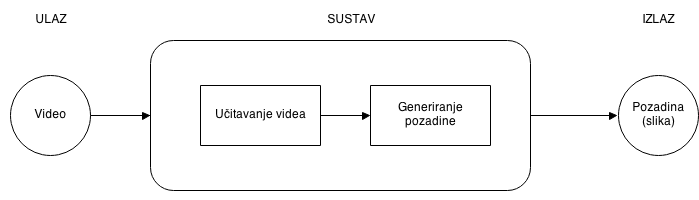
\includegraphics[height=3cm]{Dijagram1.png}
\caption{Izlučivanje pozadine}
\label{fig:sintaksno_stablo}
\end{figure}

\begin{figure}[htb]
\centering
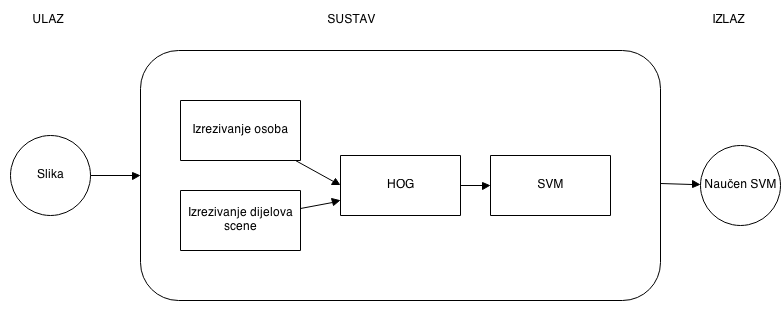
\includegraphics[height=5cm]{Dijagram3.png}
\caption{Učenje modela strojnog učenja (npr. SVM)}
\label{fig:ucenje}
\end{figure}


\begin{figure}[htb]
\centering
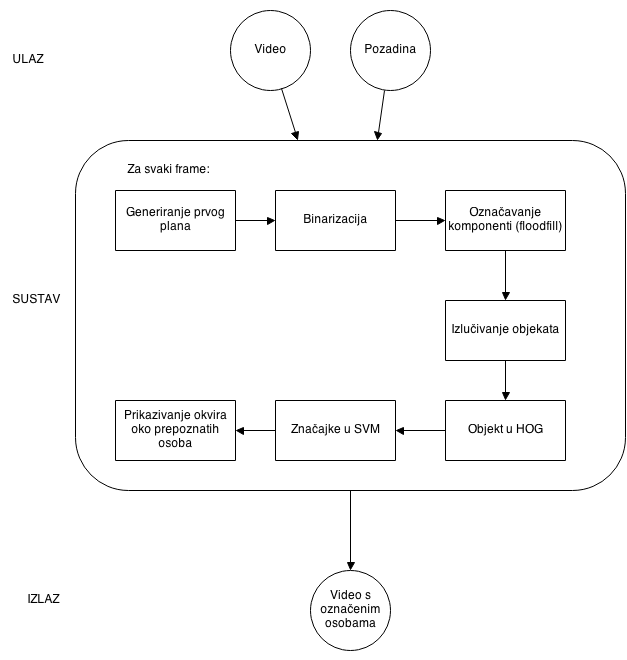
\includegraphics[width=9cm]{Dijagram2.png}
\caption{Prikaz rada sustava u realnom vremenu u modu traženja osobe na slici}
\label{fig:sustav}
\end{figure}


\chapter{Baza slika/videa}

\section{Uvod}

Za promatrani problem koristi se dvije vrste baza podataka. Prva vrsta sastoji 
se od slika, a druga vrsta od video snimaka.  

\section{Dostupne baze podataka}

\subsection{INRIA}

Baza se sastoji od slika. Navedena baza korištena je upravo za testiranje HOG 
algoritma. Podijeljena je na pozitivne (na slici se nalazi jedna ili više osoba)
i negativne (osoba na slici nema). Uz to, baza sadrži i opisnike slike koji
u sebi sadrže informaciji o pozicijama osoba na slikama. Slike su dostupne u
više različitih dimenzija (pixel x pixel): 70x134, 96x160 i 64x128.  
Baza se sastoji od ukupno 1218 negativnih primjera slika i 614 pozitivnih slika.
Za generiranje negativnih primjera negativne slike mogu se izrezivati na bilo
koji način. Nad pozitivnim slikama definirani su opisnici tako da se ukupno 
može generirati 2500 pozitivnih primjera.

\subsection{CAVIAR Test Case Scenarios}

Baza se sastoji od video snimaka. Baza je bazirana na javnim nadzornim kamerama.
Baza se sastoji od skupa ciljanih akcija osoba. Detekcija akcija nije u središtu
ovog projekta pa se mogu koristiti sve snimke ravnopravno. Dimenzija slika u 
video snimkama je 384px x 288px. Format je MPEG2 i sadrži 25 slika u sekundi.

\subsection{PETS 2009}

Baza se sastoji od slika. 
Baza je korištena za praćenje skupa ljudi pomoću nadzornih kamera. Slike su
u JPEG formatu. Dvije su različite dimenzije slika. Jedna vrsta slika dimenzija 
je 768px x 576px, a druga vrsta 720px x 576px. Svojstvo baze je da su dimenzije
osoba na slikama relativno malne s obzirom na cijelu sliku. Ovakva baza može
ispitati koliko je sustav osjetljiv na dimenzije osoba.  

\subsection{PETS 2006}

Baza se sastoji slika u JPEG formatu. Dimenzija slika je 768px x 576px i
posljedica su uzrokovanja 25 slika u sekundi. Baza je korištena za specifični 
problem praćenja ostavljene prtljage. Kako je u središtu proučavanja osoba, ova
baza pogodna je i za naš promatrani problem.

\subsection{BEHAVE}

Baza se sastoji od slika u JPEG formatu. Dimenzije slike su 640px x 480px i
slike predstavljaju slike koje su uzrokovane s frekvencijom 25 slika u sekundi.
Baza je korištena za prepoznavanje određenih ponašanja kod osoba promatranih 
nadzornim kamerama.  

\subsection{Pedestrian}

Baza se sastoji od slika u PPM formatu. Baza sadrži 924 slika. 
Slike su dimenzija 64px x 128px. Baza se sastoji od slika osoba. Procijenili 
smo da je dobra kod testiranja različitih modela strojnog učenja.

\section{Inicijalni odabir baze}

Odlučili smo odabrati jednu 
bazu podataka nad kojom ćemo promatrati problem i izraditi prototip. Odlučili
smo se za INRIA bazu zbog toga što ima opisnike osoba na slici. Zbog toga
možemo brzo izraditi primjere i testirati naš sustav.

\chapter{Programski alati}

\section{Programski jezik}
Za implementaciju sustava odabran je programski jezik python. Glavni razlog odabira jezika je lakoća pisanja programskog koda te širok izbor biblioteka u kojima su implementirani algoritmi računalnog vida. Python također sadrži veliku paletu drugih biblioteka koje nisu dostupne u nekim drugim programskim jezicima (primjerice C/C++). U konačnoj fazi projekta biti će potrebno izraditi grafičko korisničko sučelje što ne predstavlja problem jer za python postoji puno različitih frameworka koji olakšavaju tu fazu projekta. Python također omogućava pokretanje implementiranog sustava na različitim operacijskim sustavima (Windows, Linux).

\section{Biblioteke} 
Za implementaciju sustava koriste se sljedeće programske biblioteke:
\begin{itemize} 
	\item openCV
	\item scikit-image
\end{itemize}

\subsection{OpenCV}
OpenCV (Open Source Computer Vision) je biblioteka koja sadrži implementacije algoritama računalnog vida koji su namijenjeni za korištenjem u realnom vremenu. Pruža podršku i za algoritme stojnog učenja koji će biti korišteni u izradi projekta(primjerice k-NN, SVM, neuronske mreže). 

\subsection{Scikit-image}
Scikit-image je također biblioteka otvorenog koda. OpenCV više orijentiran na algoritme računalnog vida, dok scikit-image podržava više metoda za obradu slike. OpenCV podržava više programskih jezika(C++, python, Java), dok je biblioteka scikit-image namijenjena za python. Scikit-image za razliku od openCV-a za interno spremanje slika koristi numpy.ndarray. Novije verzije openCV-a također mogu koristiti numpy pa se time postiže međusobna kompatibilnost. Prednost scikit-image je lakše pisanje programskog koda i bolja razumljivost dokumentacije biblioteke. Pojedini algoritmi su implementirani unutar oba dvije biblioteke te se može uočiti bolja efikasnost openCV implementacije. Razlog tome je namjena openCV za primjenu u industriji.


\section{RapidMiner} 
RapidMiner je okruženje za strojno učenje, rudarenje podataka, itd. Alat će biti korišten za učenje, testiranje i validaciju modela koji će služiti za detekciju ljudi na video sekvencama. Alat pruža mogućnost istovremene primjene različitih postupaka učenja modela. Te na taj način možemo odabrati postupak koji daje najbolje rezultate. Dodatno podržava automatsku optimizaciju hiperparametara čime se model može dodatno poboljšati kako bi se postigli najbolji mogući rezultati. Cilj korištenja RapidMinera je pronaći najbolji model koji će kasnije biti implementiran korištenjem openCV/scikit-image biblioteka. 

\section{Repozitorij koda} 
Odabrali smo GitHub za repozitorij koda. Repozitorij koda je nužan budući da na razvoju sustava radi veći broj ljudi te postoji puno nadopuna programskog koda. GitHub pruža podršku za održavanje konzistencije i lakoću dijeljenja programskog koda. 

\chapter{Napredak projekta}

Instalirane su biblioteke i alati potrebni za izradu projekta. Napravljena su prva testiranja alata i \emph{HOG} implementacija. Ispitane različite mogućnosti obrade video snimaka. Isprobana su različita odstranjivanja pozadina i detekcija objekata na binarnoj slici. Iz baze podataka izvučene su značajke pomoću \emph{HOG} algoritma i isprobani različiti modeli strojnog učenja.

%\bibliography{literatura}
%\bibliographystyle{fer} %promijena za citiranje po redu ieeetr
%\bibliographystyle{ieeetr}

\begin{comment}
\begin{sazetak}
Simbolička regresija je postupak otkrivanja matematičkog izraza u skupu podataka. Daje se pregled metoda za simboličku regresiju s naglaskom na genetsko programiranje. Obrađuju se problemi kao što su domene funkcija (nisu definirane na cijelom skupu realnih brojeva). Problemi se rješavaju intervalnom aritmetikom i linearnim skaliranjem. Na kraju se ukratko opisuje mogućnost paralelizacije i primjene. 

\kljucnerijeci{genetsko programiranje, s}

\end{sazetak}

% TODO: Navedite naslov na engleskom jeziku.
\engtitle{Application of graphics coprocessors for program execution on stream programming model}

\begin{abstract}


\keywords{GPU, StreamIt, Sponge, StreamGate, CUDA, stream model, filter, optimization, graphics card}
\end{abstract}
\end{comment}

\end{document}
